\chapter{Resultados}
\label{chap:resultados}

Implementamos o modelo produzido utilizando a linguagem de programação \textit{C++11} \cite{c++} em conjunto com o \textit{QT 5.2.1} \cite{qt} e o \textit{solver CPLEX 12.6.1} da \textit{IBM} \cite{ibmcplex} afim de avaliar o desempenho do modelo para instâncias de diferentes tamanhos. Escolhemos a linguagem \textit{C++} para preparar as instâncias para o \textit{CPLEX} por conta do seu alto desempenho. Utilizamos as bibliotecas de acesso aos dados do \textit{QT}, por apresentarem facilidade de uso. O \textit{CPLEX} foi utilizado por se tratar de um \textit{solver} robusto, que realiza de forma automática a conversão de restrições não lineares para restrições lineares e dá suporte a execução paralela (\textit{threads}), ambos recursos utilizados nos experimentos deste trabalho.

Todos os experimentos foram realizados em um computador com processador \textit{Intel(R) Xeon(R) CPU E31240 @ 3.30GHz}, 8 GB de memória RAM e com 8 GB na partição de \textit{swap}, executando o sistema operacional Ubuntu 14.04.5 LTS.

Os testes foram realizados sobre as ofertas de disciplinas da UFC-Quixadá do semestre 2016.2. Os dados contam com 108 ofertas de disciplinas divididas em 6 cursos. São ao todo 58 professores, e a preferência de um professor por uma disciplina foi dada pelo número de vezes que esse professor ministrou essa disciplina no campus. O número de alunos nos choques de horários das disciplinas é definido de forma aleatória, já que não foi possível conseguir essas informações para os testes. Primeiramente é atribuído a cada disciplina um valor entre 10 e 50 (incluindo os extremos) referente ao número de alunos que podem cursar cada disciplina. Depois, para cada par $(a, b)$ de disciplinas, sorteamos um valor entre 0 e o mínimo do número de alunos de $a$ e $b$ para definir a interseção de alunos entre as duas disciplinas. O valor definido para a interseção passa a ser então o número de alunos que podem cursar as duas disciplinas.

A partir do conjunto de dados obtido, utilizando a linguagem de programação \textit{Python 2.7} \cite{python} para automatizar o processamento dos dados, e o banco de dados \textit{SQLite 3.11} \cite{sqlite} para armazená-los, ambos escolhidos pela facilidade de uso. Preparamos aleatoriamente instâncias com diferentes proporções dos dados reais, ou seja, instâncias com 10\%, 20\%, ..., 90\% e 100\% dos professores e disciplinas escolhidos de forma aleatória (exemplo: 10\% dos professores e 10\% das disciplinas). Aplicamos essas instâncias para valores de $\alpha \in{\{0, 0.5, 1\}}$, e definimos um tempo limite de execução de 10 horas.

É importante lembrar que as alocações produzidas com $\alpha = 1$ não levam em consideração a preferência dos professores e são possivelmente alocações indesejáveis e não aplicáveis à UFC-Quixadá. Os testes realizados para esse valor têm intuito apenas de avaliar o desempenho do modelo quando são desconsideradas as preferências por disciplinas dos professores.

A Tabela \oldref{tabela-experimentos} apresenta o resultado dos experimentos para todas as instâncias. A primeira coluna se refere ao nome das instâncias, a segunda coluna ao valor $\alpha$ aplicado sobre as instâncias, a terceira ao tempo total de execução em segundos (\textit{real time + sync time + wait time + root node processing}, fornecidos pelo \textit{CPLEX}), e a quarta coluna apresenta o resultado obtido para cada teste.

\begin{table}[h!]
	\IBGEtab{
	\Caption{\label{tabela-experimentos} Tabela de Experimentos.}
	} &   0 &     1.46 & Ótimo \\
			                      & 0.5 &     0.30 & Ótimo \\
			                      &   1 &     0.25 & Ótimo \\
			\midrule
			\multirow{3}{*}{20\%} &   0 &     3.61 & Ótimo \\
			                      & 0.5 &  1943.68 & Ótimo \\
			                      &   1 &  1353.89 & Ótimo \\
			\midrule
			\multirow{3}{*}{30\%} &   0 &    13.51 & Ótimo \\
			                      & 0.5 &  1297.13 & Solução viável (Excedeu a memória) \\
			                      &   1 &  1701.42 & Solução viável (Excedeu a memória) \\
			\midrule
			\multirow{3}{*}{40\%} &   0 &    43.79 & Ótimo \\
			                      & 0.5 &  2255.91 & Solução viável (Excedeu a memória) \\
			                      &   1 &  2043.66 & Solução viável (Excedeu a memória) \\
			\midrule
			\multirow{3}{*}{50\%} &   0 &   195.00 & Ótimo \\
			                      & 0.5 &  3405.17 & Solução viável (Excedeu a memória)\\
			                      &   1 &  8915.71 & Solução viável (Excedeu a memória)\\
			\midrule
			\multirow{3}{*}{60\%} &   0 &   170.55 & Ótimo \\
			                      & 0.5 &  8008.68 & Solução viável (Excedeu a memória)\\
			                      &   1 & 20669.59 & Solução viável (Excedeu a memória)\\
			\midrule
			\multirow{3}{*}{70\%} &   0 &   375.21 & Ótimo \\
			                      & 0.5 &  9585.77 & Solução viável (Excedeu a memória)\\
			                      &   1 &  6608.70 & Nenhuma solução (Excedeu a memória) \\
			\midrule
			\multirow{3}{*}{80\%} &   0 &  3386.09 & Ótimo \\
			                      & 0.5 & 27010.67 & Solução viável (Excedeu a memória)\\
			                      &   1 &  9018.20 & Nenhuma solução (Excedeu a memória)\\
			\midrule
			\multirow{3}{*}{90\%} &   0 &  7369.57 & Nenhuma solução (Excedeu a memória)\\
			                      & 0.5 & 10763.45 & Nenhuma solução (Excedeu a memória)\\
			                      &   1 & 10153.70 & Nenhuma solução (Excedeu a memória)\\
			\midrule
			\multirow{3}{*}{100\%}&   0 &  4611.18 & Nenhuma solução (Excedeu a memória)\\
			                      & 0.5 & 36001.29 & Solução viável (Atingiu o tempo limite) \\
			                      &   1 & 21974.03 & Nenhuma solução (Excedeu a memória)\\
			\bottomrule
		\end{tabular}%
	}{\Fonte{Produzido pelo autor}
	}
\end{table}

\newpage

Na Tabela \oldref{tabela-experimentos} podemos perceber que quando $\alpha = 0$, a implementação obteve soluções ótimas para as instâncias de tamanho até 80\% da oferta total do semestre 2016.2, mas para instâncias de maior tamanho, nenhuma solução foi encontrada. Para $\alpha = 0.5$, nenhuma solução ótima foi encontrada para as instâncias com mais de 20\% dos dados, mas obtivemos pelo menos uma solução viável para todas as instâncias com exceção da de 90\%. Para $\alpha = 1$, nenhuma solução ótima foi encontrada para as instâncias com mais de 20\%, e nas instâncias com mais de 60\% dos dados, não foi encontrada nenhuma solução viável.

Quanto às alocações geradas, nas instâncias menores ocorrem muitos casos em que professores são associados à disciplinas que estão fora da sua área de estudo, como por exemplo, um professor de otimização associado à disciplina de fotografia. Isso é esperado, pois sendo os professores e disciplinas escolhidos de forma aleatória para compor a instância, não temos a garantia de haver uma proporção adequada entre os professores de uma área de estudo e as disciplinas dessa mesma área. É importante lembrar, que essas instâncias tem o intuito apenas de avaliar o desempenho do modelo. Na solução viável encontrada para a instância com 100\% dos dados, a alocação de professores em disciplinas foi quase em sua totalidade semelhante às alocações que são aplicadas atualmente no campus. Apesar disso houveram algumas alocações aparentemente indesejáveis entre professores e disciplinas (professores alocados à disciplinas às quais não estão haptos a lecionar). Considerando que a solução encontrada não é a solução ótima, e que o programa parou por exceder o tempo limite de execução, isso já era esperado para essa situação.

Como ilustração, a Figura \oldref{figura-2} apresenta a alocação gerada para as disciplinas do quarto semestre do curso de Ciência da Computação para a instância com 100\% dos dados e $\alpha = 0.5$.

\begin{figure}[htbp]
	\centering
	\IBGEtab{
		\Caption{\label{figura-2}Alocação das disciplinas do quarto semestre do curso de Ciência da Computação}		
    }{
		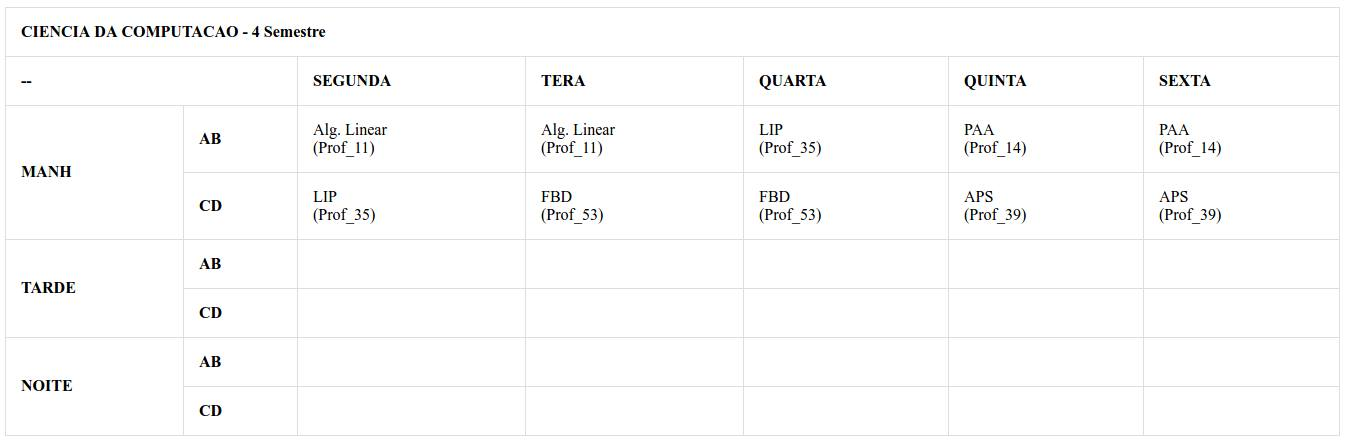
\includegraphics[scale=0.32]{figuras/alocacao}
	}{
	\Fonte{Elaborada pelo autor}
}
\end{figure}
